\documentclass[12pt,a4paper]{article}
\usepackage[utf8]{inputenc}
\usepackage[english]{babel}
\usepackage{url}
\usepackage{hyperref}
\usepackage{amsmath}
\usepackage{amsfonts}
\usepackage{amssymb}
\usepackage{graphicx}
\usepackage[left=2cm,right=2cm,top=2cm,bottom=2cm]{geometry}
\usepackage[style=authoryear,sorting=nty]{biblatex}
\addbibresource{literatur.bib}
\author{Johannes Walter}
\newcommand{\indep}{\perp \!\!\! \perp}

\usepackage{xcolor}
\hypersetup{
    colorlinks,
    linkcolor={red!50!black},
    citecolor={blue!50!black},
    urlcolor={blue!80!black}
}

\begin{document}

\begin{titlepage}
    \centering
    \vspace{5cm}
    {\scshape Centre for European Economics Research \par}
    \vspace{0.5cm}
    {\scshape Research Proposal Summer School Revealed Preferences \par}
    \vspace{1.5cm}
    {\scshape\LARGE Revealed Preferences under Framing: Users valuation of privacy \par}
    \vspace{2cm}
    {\itshape Johannes Walter \par}
    \vspace{1cm}
    \begin{abstract}
    Diese Dokumentation enth"alt eine sortierte Liste der wichtigsten
    \LaTeX--Befehle. Die einzelnen Listeneintr"age sind untereinander
    durch viele Querverweise verkettet, die ein Auffinden inhaltlich
    zusammengeh"origer Informationen erheblich erleichtern.
    \end{abstract}
    \vfill
    Summer School Revealed Preferences \par 
    Nicolai Kuminoff 
    \vfill

    % Bottom of page
    {\large \today\par}
\end{titlepage}


\section{Introduction}
\label{introduction}
Idea: 
\begin{itemize}
    \item Topic: Revealed preferences and privacy
    \item Advantage of this approach: connects RP and my field of Digital Econ
    \item Setting: GDPR introduced choice on cookies. Cookies choice depends on framing. This new model in the JPE can factor in framing. We can then derive people's revealed preference for privacy
    \item Data: Collect browsing behavoir from random sample. Requirement: Browser add-on. I can refer to the Paper from the conference.
    \item Model: From the JPE Paper, that's gonna be nice
    \item Intro: Science article, put it in general  context of revealed preference research on privacy. If it doesn't exist yet, great (but unlikely). If it does already exist, I'd wager nobody so far has considered the effects of framing with this new model.
\end{itemize}

\section{Economic Model}
\label{model}
The description of this model follows chapter one of \textcite{acquisti2015privacy}. A fully detailed description 
of the model can be found there and is beyond the scope of this research proposal. Here, only the main concepts 
necessary for understanding this proposal are presented.

\subsection{Basic model notation}

A decision maker i chooses from a binary decision set $ \textbf{S} = \lbrace 0,1 \rbrace  $ und two possible frames $ D_{i} \in \lbrace 0,1 \rbrace $. 
In the context of this research proposal, the decision coded with a $0$ 
could refer to an individual's decision to accept only technically necessary cookies and 
the decision coded with a $ 1 $ could refer to an individual's decision 
to allow for non technically necessary cookies. Frame $ 0 $ could be the situation where the default setting is such that 
technically necessary cookies are the only pre-chosen ones and the user would have to actively engage in clicking on all non-technically necessary 
cookies she wishes to allow. Frame $ 1 $ could then refer to the situation 
where in the default setting both types of cookies are pre-chosen and the user accepts both types with one click. We can adapt a notation that is akin to what many researchers like to use in a potential outcome setting. $ Y_{i}(0) $ and $ Y_{i}(0) $ denotes then the decision individual i makes under frame $ D_{i} = 0 $ and $ D_{i} = 1 $, respectively.
Decision makers are assumed to have strict ordinal preferences over the set of available options. $ Y^{*}_{i} \in \lbrace 0,1 \rbrace $ denotes the most preferred option.
Each decision maker is characterized by a vector of random variables 
$ (Y_i(0), Y_i(1), D_i, Y^*_i) $, which are drawn from an underlying population distribution.
For each $ i $, the researcher observes the pair $ (Y_i, D_i) $, where 
$ Y_i = Y_i(0)D_i + Y_i(1)(1-D_i)$. \textcite{goldin2020} assume for their model 
that the researcher does not observe $ Y^*_i $ and only observes one of $ Y_i(0)$ and $ Y_i(1)$, depending on the frame $D_i$.

The data that is suggested to be collected in this proposal deviates
in a crucial way from this assumption. In contrast to the datasets \textcite{goldin2020}
have in mind, the dataset in this proposal will contain \textit{repeated} observations of the same individual. 
The number of observations for each $ i $ can be denoted with a subscript 
$ k \in \lbrace 1,\dots, K \rbrace $ such that $ Y_{i, k} $ is observed. 
Importantly, here it is assumed that $ K $ is sufficiently large to allow for at 
least one observation of each framing $ D_{i} \in \lbrace 0,1 \rbrace $.

The mean choices among decision makers assigned to a frame is denoted by 
$ \bar{Y}(1) \equiv E[Y_i | D_i = 1]  $ and $ \bar{Y}(0) \equiv E[Y_i | D_i = 0]  $.

\textcite{goldin2020} continue their description of the model as follows: Each
decision maker can choose either consistently, i.e. the same choice under each frame,
or choose in a way that is responsive to the frame. Consistency is denoted by $ C_i = 1 $ iff $Y_i(0) = Y_i(1) $ else $C_i = 0 $.
Again, they assume that each $ i $ is observed only under one frame, such that $C_i$ is not observed.
In the context of this proposal, as described above, it is assumed that each $ i $ is observed under both frames, such that
$ C_i $ is identified. This difference is crucial for one of the main contributions of this proposal.
The additional information in this dataset allows to calculate two sets of results. For the first one, the additional information in this dataset is not used.
The analysis will proceed under the assumption of \textcite{goldin2020}. The second set of results will be obtained using the full amount of information
in the dataset. As such, the "ground-truth" that remains hidden under \textcite{goldin2020}'s assumptions, is observed. In other words, with the dataset proposed 
here, it will be able to identify all individuals who make consistent choices, independent of the frame. 
Having these two sets of results, one can compare the estimates from both to arrive at an assessment of the quality of \textcite{goldin2020}'s model accuracy.

%HERE IT is necessary to say which observations to use if there is a conflict!
% Random subsample vs. drop the inconsistent ones

\subsection{Model assumptions}

One of \textcite{goldin2020}'s main contributions is to make the necessary assumptions for their analysis explicit.
Furthermore, the assumptions are fundamental to their approach and will be required in section \ref{data and methods} to
derive framing-consistent estimates for the entire population.
For these reasons, the assumptions will be presented shortly here as well.
Each assumption is first presented in the way \textcite{goldin2020} lay them out and subsequently
followed by a comment on how each assumption relates to the approach suggested in this research proposal.

\begin{itemize}
    \item Assumption A1) \textit{Frame separability}: For all $ i, Y^*_i $ does not depend on $D$.
\end{itemize}

For each individual, the most preferred option does not depend on the framing.
This is an assumption about the content of a decision makers' preferences and is 
useful to define which features of the environment are considered to be part of the framing \parencite[p. 2764]{goldin2020}.

\begin{itemize}
    \item Assumption A2) \textit{Frame exogeneity}: $ (Y_i(0), Y_i(1), Y^*_i) \indep D_i$.
\end{itemize}

This assumption refers to the data generating process by which decision makers are assigned to frames.
It is similar in nature to the assumption in the potential outcome setting that says treatment and
assignment to treatment need to be independent. A2) makes sure that observed differences
are due to the effect of the frames, rather than due to differences in the groups of individuals assigned
to each frame.

\begin{itemize}
    \item Assumption RPA) \textit{Revealed-preference assumption}: For all $ i, Y^*_i = Y_i $.
\end{itemize}

In \textcite{goldin2020}'s setting, a framing effect is observed when assumptions A1) and A2)
are satisfied and one observes $\bar{Y}(1) \neq \bar{Y}_i $. In the context
of this research proposal, a framing effect occurs if $ Y_{i, k}(0) \neq Y_{i, \lnot k}(1)$ for
at least one $k$.

\begin{itemize}
    \item Assumption A3) \textit{Consistency Principle}: For all $ i, C_i = 1 \Rightarrow Y_i = Y^*_i $.
\end{itemize}

This assumption tells us that preferences are only guaranteed
to be revealed by choices for those decision makers who choose consistently across frames.
This assumption also applies in the context of the data that this research proposal suggests.
% What if there is not a single one who is consistent?!

\begin{itemize}
    \item Assumption A4) \textit{Frame monotonicity}: For all $ i, Y_i(1) \geq Y_i(0) $.
\end{itemize}

Assumption A4) allows \textcite{goldin2020} to recover aggregate information
about consistency despite the fact that $ C_i $ is not observable on the individual level in their setting. The assumption
requires that when a frame does affect choices, it does so in the same
direction for each affected decision maker.
Since $ C_i $ can be observed directly in the setting of this proposal, A4) is not necessary for the analysis of this
dataset.

\section{Data and Methods}
\label{data and methods}
Subsection \ref{data coll} describes how the data is proposed to be collected and the kind of data that will be collected.
It will also contain a short overview of
browser cookies and their functionality. Section \ref{method} will present how
\textcite{goldin2020} identify their parameters of interest and the simplifications
that are possible when one has access to a richer dataset, as proposed here.

\subsection{Data} \label{data coll}
The process of data collection is inspired by \textcite{levy2020}. In this paper, the
author wrote a browser extension for Google's Chrome browser. Via a Facebook ad campaign,
8084 participants for a survey were attracted. At the end of the survey, they were offered a
small reward in exchange of installing the browser extension on their device \parencite[p. 9]{levy2020}.
2262 survey participants installed the extension, and 1835 kept the extension installed for at least two weeks.

This research proposal suggests to apply the same design. Participants can be attracted
via a Facebook or Google ad campaign. In a short survey, their age, gender and nationality could
be elicited (for analysis of heterogeneity and the selection on observables identification approach as described in section \ref{method}). Afterwards, they are asked to install a small browser extension in exchange for
a reward. The extension will use a short javascript code that writes a log file. This log file will keep track of whether a participant has 
visited a website that asks for cookie settings. It will also log whether
the default setting is to accept all cookies, or whether by default only the technically necessary cookies are selected.
Importantly, the extension needs not collect any information about the content of the visited websites. From a privacy point of view,
this design is less invasive than the one in \textcite{levy2020}. This observation motivates the assumption that there is a sufficient amount of people who are willing
to participate in such a study.
%Chrome makes it easy to include extensions
% Talk about the money required
\\
\\
A hypertext transfer protocol (HTTP) cookie is a small piece of data that is sent from
a website and stored on a users device. For the purposes of this research proposal, cookies can be classified into two groups. First, there are
technically necessary cookies that ensure a website is working as intended. Such cookies could remember preceding user
interactions with the site, e.g. adding an item to a shopping cart, or logging in. Second, there are cookies that are not technically
necessary to ensure the website's functionality. A common example are for example third-party tracking cookies which record previously visited websites.
These non-essential third-party tracking cookies can generate long-term records of a user's browsing history and can therefore manifest a potential privacy concern.
Websites have an incentive to allow these cookies, as they receive third-party payments in return (common tracking cookies are e.g. Google AdSense or Facebook remarketing).  
The GDPR requires that all websites which target European Union or European Economic Area member states ask their users for consent
before they are allowed to store non-essential cookies on a user's device. The host of a website still
has a choice on how to frame this question. Either non-essential cookies are unselected by default and if the
user clicks once on "accept" no tracking is possible. Or non-essential cookies are selected by default and if the user wants
to avoid them it is necessary to go into the website's privacy settings and unselect tracking cookies manually.
%order and at least one observation of each kind

\subsection{Method} \label{method}

This section will describe how \textcite{goldin2020} identify their model parameters. It will also contain a description
of how the parameter identification is simplified by the dataset suggested in this research proposal.

In the first step, \textcite{goldin2020} focus on the consistent decision makers, i.e. the subgroup of individuals
whose decision does not depend on the frame. With a dataset as suggested in this proposal, it is trivial to find this group. All decision makers who are not influenced by the framing belong to the consistent decision makers
(it is, of course, possible that there zero decision makers in the dataset, which would be an interesting result in itself). 
Once the consistent decision makers are found, using assumption A3), the consistency principle, the options they preferred can be found.

\textcite{goldin2020}'s method is also applicable to datasets that do not contain repeated observations for each individual.
It is worth noting, that \textcite{goldin2020} mention that their method can also improve datasets that do contain repeated observations.
In particular, this is the case when the \textit{order} in which the repeated observations are generated can itself be considered a framing. 
For instance, this could be an issue if researchers were to analyse survey data, where the questions were not sufficiently randomized. 
For the dataset that is described in section \ref{data coll} the order in which individuals see each question about cookies is assumed to follow a random process.

\textcite{goldin2020} continue by describing the conditions for which consistent decision makers preferences can be identified when each decision maker
is observed under a single frame. 

\begin{itemize}
    \item Proposition 1: $ \bar{Y}_C \equiv \bar{Y}(0)/(\bar{Y}(0) + 1 - \bar{Y}(1))$
    \item Proposition 1.1: Under assumptions A1 - A4, $ E[Y^*_i | C_i = 1] = \bar{Y}_C $.
    \item Proposition 1.2: Under assumptions A1 - A3, $ \bar{Y}_C \geq 1/2 \Rightarrow \bar{Y}_C \leq E[Y^*_i | C_i = 1] \leq 1$, and $\bar{Y}_C \leq 1/2 \Rightarrow 0 \leq E[Y^*_i| C_i = 1] \leq \bar{Y}_C$.
\end{itemize}

Proposition 1.1 follows from the insight that, given frame monotonicity, only consistent decision-makers choose against the frame \parencite[p. 2768]{goldin2020}.
Proposition 1.2 provides a partial identification result, as it defines upper and lower bounds for the fraction of frame consistent decision makers. The results under 
proposition 1.2 are robust to failures of frame monotonicity. In other words, it guarantees bounds in cases when there are decision makers
who decide against the frame, but are still in truth inconsistent. These decision makers are defined by \textcite[p. 2768]{goldin2020}
as frame defiers.

The logic of proposition 1 is illustrated in table \ref{table}, which is taken from \textcite[p. 2769]{goldin2020}. To understand this table, it is important to 
know the conditions that produced the data. Here it is assumed that the researchers observe answers under both types of framing. Yet each individual's answer is only
observed once under one type of framing.
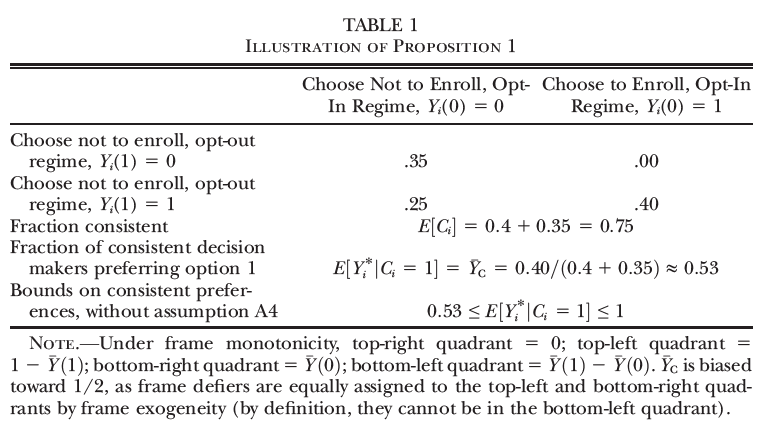
\includegraphics{table.png} \label{table}
\\
\\
To the best of my understanding, the table contains a mistake. I believe that the description for the second row of the table should read
"Choose to enroll, opt-out regime, $ Y_i(1) = 1$" (instead in the version in the article, the description mistakenly contains a "not": "Choose \textbf{not} to enroll, opt-out regime, $ Y_i(1) = 1$").

It becomes easy to see how the fraction of consistent decision makers can be found even if each decision makers is only observed under one frame.
In the example in table \ref{table}, 0 \% of observations fall into the top-right quadrant by assumption.
The top-left quadrant is the result of $1-\bar{Y}(1)$, where $\bar{Y}(1)$
is the fraction of decision makers who chose to enroll under the opt-out framing. This number is observed by the researchers.
The bottom left quadrant is the difference between the fraction of decision makers who enroll under opt-out framing and the fraction
of decision makers who enroll under opt-in framing. Both fractions are observed.
The bottom right quadrant is the fraction of decision makers who enroll under opt-in framing, which is, again, observed.
Now the fraction of consistent decision makers who prefer option 1 can be calculated according to proposition 1. When assumption A4 is relaxed,
at least a lower bound can be calculated.
This way, despite the researcher not observing each decision maker under each framing, the preferences of the consistent decision makers can be recovered.

When a researcher has access to a dataset as proposed in this research proposal, the fraction of consistent decision makers preferring
option 1 can be calculated directly and could be compared to the result from \textcite{goldin2020}'s method (in table \ref{table} approximately 53\%). Thus, providing
a way to check the method for its validity and precision in a certain setting.
 % Why is this not sufficient?! Find place in paper
\\
\\
For completeness, the following paragraph will shortly describe the three methods \textcite[p.2769]{goldin2020} suggest to extrapolate the preferences from the consistent decision makers
to the rest of the population.  As this part is not the focus of this research proposal only the main ideas are introduced here. For a detailed discussion, see \textcite[p.2767]{goldin2020}.

\textcite{goldin2020} suggest three different ways to proceed.
The first approach they present explores what can be said abut they entire population without assuming additional  behavioral assumptions.
Without further assumptions, population preferences can only be obtained as one-directional bounds \parencite[p. 2772]{goldin2020}. 
The second approach is known from the sample-selection literature: adjusting for observables as individuals "select" into the group of consistent decision makers.
In order for this approach to result in unbiased estimates, it is necessary to assume that all the relevant variables that link the
correlation between preferences and consistency are observed by the researcher. And finally, \textcite{goldin2020} introduce an instrumental variable based approach, 
which they call \textit{decision-quality instrument}. Such an instrumental variable is a part of the decision architecture affecting   
only the decision makers' consistency and has no relationship with the decision maker's preferences.




% 1. Identify the subgroup of consistent decision makers
% 2. Project from that subgroup onto the entire Population
%     2.1 Partial Identification
%     2.2 Selection on observables
%     2.3 Instruments

%     To illustrate
%     the notation with the privacy example from the introduction, let Yi indicate
%     whether i allows a company to use her data, Di 5 1 indicate the optout
%     regime, and Di 5 0 indicate the opt-in regime, so that Y ð1Þ 5 0:65
%     and Y ð0Þ 5 0:40.   

%A) Data
%Komplettes Deaktivieren der Cookies in Firefox oder Cookies deaktivieren für nutzungsbasierte Online-Werbung
%https://www.bild.de/wa/ll/bild-de/privater-modus-unangemeldet-54578900.bild.html

%By using our site, you acknowledge that you have read and understand our Cookie Policy, Privacy Policy, and our Terms of Service
%https://tex.stackexchange.com/questions/823/remove-ugly-borders-around-clickable-cross-references-and-hyperlinks

%I observe whether individual i accepts all cookies or only the technically necessary ones $(Y_{i})$, and whether the default is opt-in $ (D_{i} = 0) $ or opt-out $ (D_{i} = 1) $ at the date of visitng the website. 
%Through an additional survey, we also observe age, sex and race for each employee.

%B) Recovery of Consistent Preferences

%\begin{itemize}
%    \item Under assumptions A1 - A4, proposition 1 allows us to identify the preferences of the consistent visitors
%    \item A1) requires that the preferences over the cookie choice do not depend on opt-in or opt-out.
%    \item A2) Frame exogeneity
%\end{itemize}

%Under A)1 to A4), we identify the preferences of the consistent decision makers.
%What you get is the preference of the consistent decision-makers.

%C) Recovery of the Population Preferences

%Subsection 2) Identification and identification of popuilation preferences

%Explain how the original model arrives at estimates and how it extrapolates. If this takes too long and is too difficult, just make it top level and refer to the paper for details

%Cookies: 

%\begin{tabular}{p{0.4\textwidth}|p{0.4\textwidth}}
%    %%%
%    Technically necessary cookies & Technically non-necessary cookies \\
%    \hline
%    \hline
%    \begin{itemize}
%      \item I
%      \end{itemize}
%     &
%      \begin{itemize}
%      \item Sample Text
%      \item Sample Text
%    \end{itemize}\\
%    %%%
%    \begin{itemize}
%      \item Sample Text
%      \item Sample Text
%      \end{itemize}
%      &
%      \begin{itemize}
%      \item Sample Text
%      \item Sample Text
%    \end{itemize}
%    %%%

%   \end{tabular}

\printbibliography


\end{document}